\subsection{m6i family}
It is worth exploring whether, and to what extent, the behavior we witnessed for the m5 family 
is present on the m6i family. The m6i family runs on the 3rd Generation Intel Xeon Scalable 
processor. We investigated the maximum performance degradation that can happen on the test nodes 
from adding idle and busy VMs with different instance types. Table \ref{tab::max_m6i} summarizes
the results.
\begin{table}[H]
\begin{center}
\begin{tabular}{ |c|c|c|c|c|c }
 Instance type & large & xlarge & 2xlarge & 4xlarge \\
 \hline
 Maximum Nodes & 64 & 32 & 16 & 8  \\
 \hline
Degradation (Busy) \% & 1.48 & 1.6 & 1.74 & 2.3  \\ 
\hline 
Degradation (Idle) \% & 0.05 & 0.06 & 0.06 & 0.07  \\ 
\end{tabular}
\end{center}
\caption{Maximum achievable performance degradation on our test node across various m6i instance types}
\label{tab::max_m6i}
\end{table}
\noindent
The difference from the previous experiments with the m5 family is that we notice a difference between 
adding idle or busy neighbors. Adding idle neighbors always results in a sub 0.1\% performance 
degradation which is practically insignificant. This difference between busy and idle instances can't be 
assigned to hypervisor overhead alone as we notice a sub 0.1\% overhead when adding busy instances
on the m6g dedicated host that uses the same Nitro v2 Hypervisor, as Table \ref{tab::max_m6g} shows.\\
These results can be misleading in 
suggesting that the performance degradation for the m6i family. 
However, in these experiments, all the instance types started from nearly the same nominal performance 
level, which is roughly 2\% away from the "worst" runtime possible on the metal instance (128 busy 
threads). This explains the small levels of performance degradation we witnessed in comparison to the m5 family 
where the m5.large and m5.xlarge instances started with a relatively better (nominal) performance than 
the other types resulting in a bigger performance degradation in comparison to the other types. 
We now analyze the execution runtime of busy threads directly on the m6i.metal instance, in comparison
to to the test node while adding busy 4xlarge neighbors. 
\begin{figure}[H]
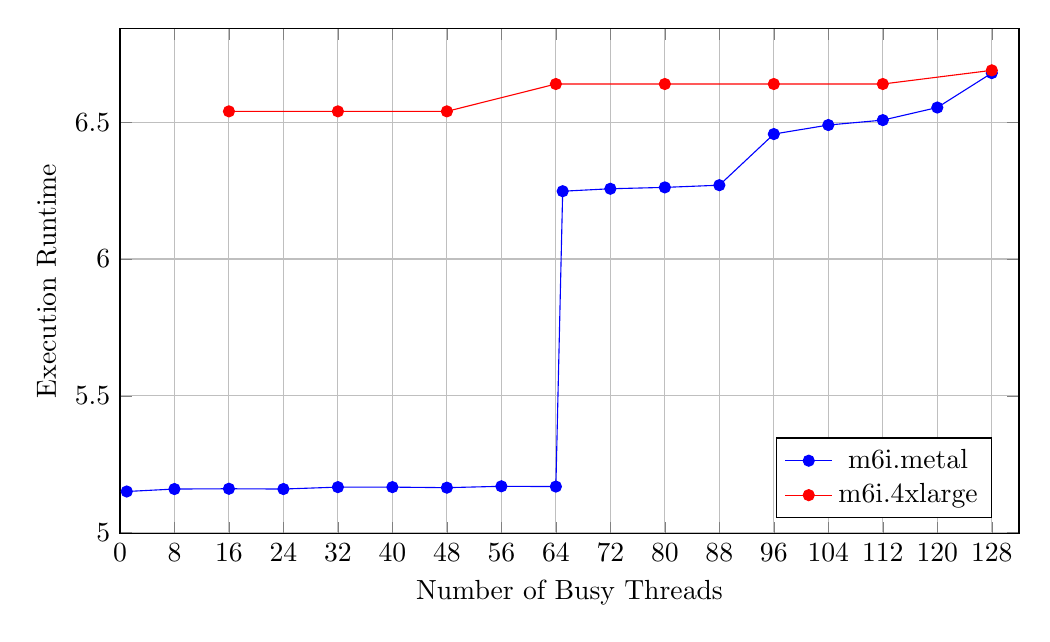
\begin{tikzpicture}
  \begin{axis}[
    width=13cm,
    height=8cm,
    ylabel={Execution Runtime},
    xlabel={Number of Busy Threads},
    grid=major,
    xmin=0, 
    xmax=132,
    xtick distance= 8,
    legend pos=south east
  ]
    \addplot[
      color=blue,
      mark=*,
    ]
    coordinates {
      (1, 5.150)
      (8, 5.159)
      (16, 5.160)
      (24, 5.159)
      (32, 5.166)
      (40, 5.166)
      (48, 5.164)
      (56, 5.169)
      (64, 5.168)
      (65, 6.248)
      (72, 6.257)
      (80, 6.262)
      (88, 6.270)
      (96, 6.457)
      (104, 6.490)
      (112, 6.508)
      (120, 6.554)
      (128, 6.68)
    };

    \addplot[
      color=red,
      mark=*,
    ]
    coordinates {
      (16, 6.54)
      (32, 6.54)
      (48, 6.54)
      (64, 6.64)
      (80, 6.64)
      (96, 6.64)
      (112, 6.64)
      (128, 6.69)
    };
\addlegendentry{m6i.metal}
\addlegendentry{m6i.4xlarge}

\end{axis}
\end{tikzpicture}
\caption{Performance of the test node in comparison to running the threads natively on m6i.metal}
\end{figure}
\noindent
At 128 threads, both the m6i metal and the 
test nodes had the same execution runtime, which further supports the claim that the difference between 
busy and idle neighbor in Table \ref{tab::max_m6i} is not solely due to hypervisor overhead.  
We notice the same behavior we witnessed on 1st gen and 2nd gen Intel Xeon Scalable processor from the 
m5.family. We notice that in both the m5.metal and m6i.metal, the most significant performance degradation 
happens exactly at    \begin{math}n / 2 + 1\end{math} with n being the maximum number of vCPUs available 
to the dedicated host. Our hypothesis is that the first \begin{math}n/2\end{math} threads are scheduled 
each on an independent physical core. However the \begin{math}n / 2 + 1\end{math} thread needs to share 
a physical core with another thread, as explained previously. This results in the performance degradation 
of 20.9\% we witness here and 25.22\% using m5.metal. The maximum performance degradation using this 
m6i.metal is less than m5.metal, reaching 31.85\% here in comparison to 53\%. Over the first 64 
threads (\begin{math}n/2\end{math}), we notice very small performance degradation of 0.35\%, in 
comparison to 13.2\% on the m5.metal instance (over the first 48 threads). In this experiment as well, 
we notice that the the first m6i.4xlarge has an intial performance 26.7\% worse than deploying the 
threads natively on the bare-metal instance. We assume that the same vCPU distribution happens with this 
host as explained for the m5 host. \\
We investigate whether this behavior is also present on processors from other vendors 
that support \ac{SMT}, such as certain AMD models.
